%Lernziele Folie 1
\begin{frame}
    \b{ \frametitle{Einführung}
        \begin{Lernziele}{Halbleiter}
            \title{Lernziele: Halbleiter}
            Die Studierenden können
            \begin{itemize}
                \item Zusammenhänge zwischen Festkörpern und dem Bändermodell erklären.
                \item Vorgänge innerhalb von Halbleitern beschreiben.
                \item verschiedene Halbleitermaterialen und deren Eigenschaften bennen.
            \end{itemize}
            \end{Lernziele}   
    }
\end{frame}

%Einführung
\begin{frame}
     \b{\fta{Einführung}
     \begin{figure}[H]
        \centering
        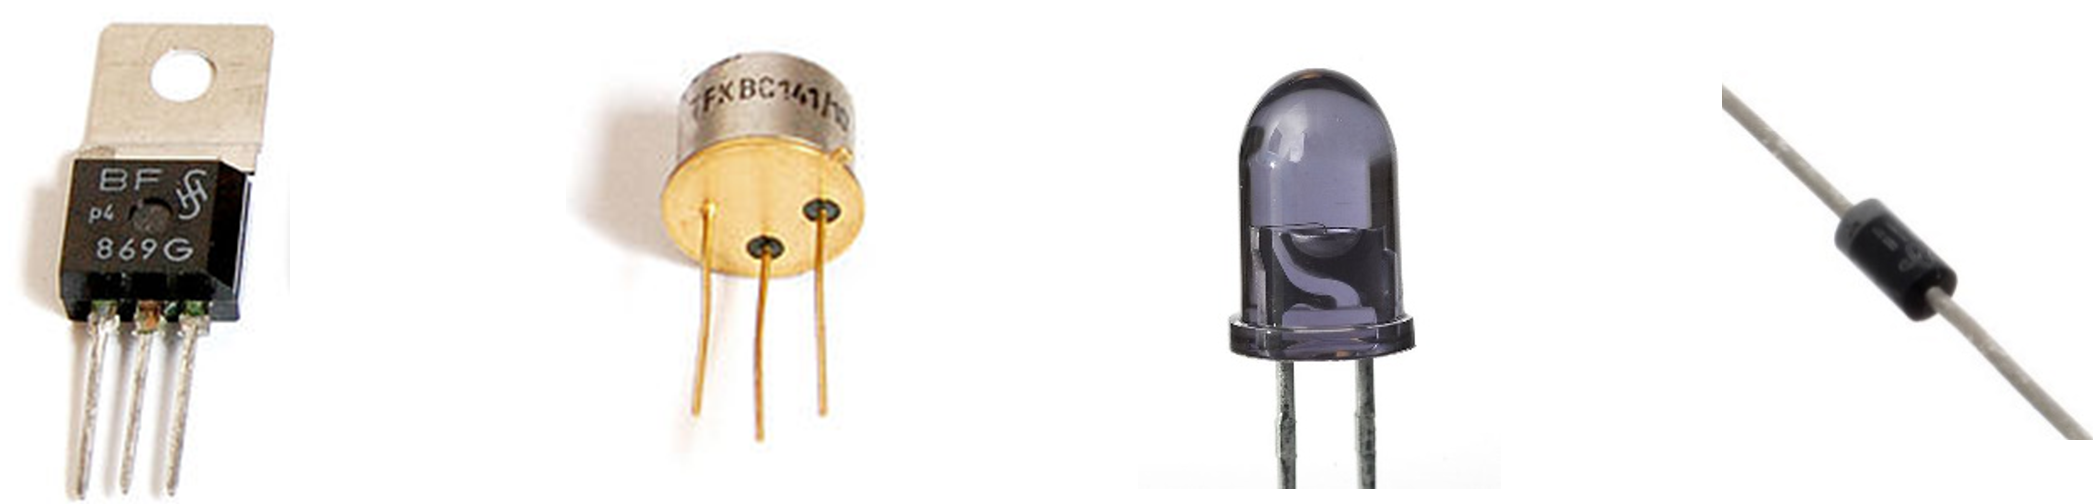
\includegraphics[width=.8\textwidth]{Bilder/kap1/AufnahmenHalbleiterWiki.png}
        %\caption{\textbf{Beispielfotos typischer Halbleiterbauelemente.} V.l.n.r.: Feldeffekttransistor, Bipolartransistor, Leuchtdiode, Diode.}  
        %\label{fig:BeispielfotosVerbreiteterHalbleiterbauelemente}
    \end{figure}
     }
% %Gesprochener Text:
% %speech{Einführung Halbleiterbauelemente}{1}{Halbleiterbauelemente sind das Rückgrat der modernen Elektronik und entscheidend für die Funktion vieler elektronischer Geräte, von Computern und Mobiltelefonen bis hin zu Solarzellen. Diese Bauelemente nutzen die besonderen Eigenschaften von Materialien, die weder gute Leiter noch gute Isolatoren sind, sondern dazwischen liegen, die sogenannten Halbleiter. Der Text beschreibt zunächst ihre Funktionsweise mit dem Bändermodell, das die elektronischen Zustände in Festkörpern erklärt, und untersucht dann verschiedene Halbleitermaterialien, ihre Eigenschaften und Anwendungen. Ein Schlüsselkonzept ist der pn-Übergang, der die Basis für viele Bauelemente bildet. Im zweiten Teil werden verschiedene Halbleiterbauelemente wie Dioden und Transistoren und deren Funktionen erläutert.}}
\end{frame}

\begin{frame}
\b{\fta{Einführung}
\begin{itemize}
    \item Halbleiterbauelemente sind zentral für die Funktion zahlreicher elektronischer Geräte wie Computer, Mobiltelefone und Solarzellen.
    \item Sie basieren auf Materialien, die weder gute Leiter noch gute Isolatoren sind. Ihre Funktionsweise kann mithilfe des Bändermodells erklärt werden.
    \item In diesem Kapitel werden die Grundlagen der Halbleitertechnik erläutert.
\end{itemize}}
% %Gesprochener Text:
% %speech{Einführung Halbleiterbauelemente}{1}{Halbleiterbauelemente sind das Rückgrat der modernen Elektronik und entscheidend für die Funktion vieler elektronischer Geräte, von Computern und Mobiltelefonen bis hin zu Solarzellen. Diese Bauelemente nutzen die besonderen Eigenschaften von Materialien, die weder gute Leiter noch gute Isolatoren sind, sondern dazwischen liegen, die sogenannten Halbleiter. Der Text beschreibt zunächst ihre Funktionsweise mit dem Bändermodell, das die elektronischen Zustände in Festkörpern erklärt, und untersucht dann verschiedene Halbleitermaterialien, ihre Eigenschaften und Anwendungen. Ein Schlüsselkonzept ist der pn-Übergang, der die Basis für viele Bauelemente bildet. Im zweiten Teil werden verschiedene Halbleiterbauelemente wie Dioden und Transistoren und deren Funktionen erläutert.}}
\end{frame}

%Zusammenhang Bohrsche Atommodell und Bändermodell.
\begin{frame}
\b{\begin{columns}
    \frametitle{Das Bändermodell}
    \column[c]{0.3\textwidth}
    \begin{figure}[H]
        \onslide<1->{
        \begin{minipage}[t]{0.48\textwidth}
            \begin{figure}[H]
                \centering
                \includesvg[width=1\textwidth]{Bilder/kap1/ZusammenhangBohrscheAtommodellundBaendermodell/ZusammenhangBohrscheAtommodellundBaendermodell_1}
            \end{figure}
        \end{minipage}
} \onslide<2->{
        \begin{minipage}[b]{0.48\textwidth}
                \begin{figure}[H]
                \centering
                \includesvg[width=1.1\textwidth]{Bilder/kap1/ZusammenhangBohrscheAtommodellundBaendermodell/ZusammenhangBohrscheAtommodellundBaendermodell_2}
            \end{figure}
        \end{minipage}
}
        %\caption{\textbf{Zusammenhang zwischen dem Bohrschen Atommodell und Bändermodell.} Darstellung des Zusammenhangs 
                %zwischen dem Abstand von Elektronen zum Kern und Höhe des zugehörigen diskreten Energieniveau. Links: Bohrsche 
                %Atommodell eines Si-Atoms. Rechts: Bändermodell eines Si-Atoms mit den möglichen Energieniveaus.}  
        %\label{fig:ZusammenhangBohrschesAtommodellUndBaendermodell}
    \end{figure}
    \column[c]{0.6\textwidth}
        \begin{itemize}
            \onslide<1->{
            \item Das Bändermodell beschreibt die elektronischen Eigenschaften von Festkörpern und ordnet die Energiezustände von Elektronen in Energiebänder.}
            \onslide<2->{
            \item Es hilft, elektrische, optische und magnetische Eigenschaften von Materialien zu verstehen und zu erklären.}
            \onslide<3->{
            \item Das Modell ermöglicht die Erklärung von Leitung, Isolation, Halbleiterverhalten sowie Oberflächen- und Grenzflächenzuständen.}
            \onslide<4->{
            \item In der Abbildung auf der linken Seite ist der Zusammenhang zwischen bohrschem Atommodell und Bändermodell illustriert.}  
        \end{itemize}
    \end{columns}
}
%Gesprochener Text:
%speech{Einführung Halbleiterbauelemente}{1}{Das Bändermodell ist ein grundlegendes Konzept in der Festkörperphysik, das die elektronischen Eigenschaften von Festkörpern beschreibt. Es bietet die theoretische Grundlage, um die elektrischen, optischen und magnetischen Eigenschaften von Materialien zu verstehen. Das Modell ordnet die Energiezustände von Elektronen in sogenannte Energiebänder, die das elektronische Verhalten des Materials maßgeblich beeinflussen. Mit dem Bändermodell lassen sich komplexe Phänomene wie Leitung, Isolation, Halbleiterverhalten sowie die Bildung von Oberflächen- und Grenzflächenzuständen erklären. Im nächsten Abschnitt werden die Grundprinzipien des Modells und der Ladungsträgertransport detailliert erläutert.
%Das Bohrsche Atommodell hingegen nimmt an, dass die Energieniveaus von Elektronen in einem Atom diskret sind. Laut diesem Modell bewegen sich Elektronen auf definierten Bahnen um den Atomkern, die als Schalen bezeichnet werden. Jede Schale hat ein charakteristisches Energieniveau, das in Bezug auf den Abstand vom Atomkern quantisiert ist. Elektronen in den inneren Schalen haben niedrigere Energieniveaus als die in den äußeren Schalen. Der Zusammenhang zwischen dem Bohrschen Atommodell und dem Bändermodell wird in Abbildung 2 gezeigt.}}

\end{frame}

%UebergangVonEnergieniveausZuBaendern
\begin{frame}
    \b{
    \frametitle{Das Bändermodell}
    \begin{figure}[H]
        \centering
        \includesvg[width=\textwidth]{Bilder/kap1/UebergangVonEnergieniveausZuBaendern}
        \caption{\textbf{Übergang von Energieniveaus zu Bändern} Zusammenhang zwischen den möglichen Energiezustände in Abhängigkeit zur Anzahl der Atome. V.l.n.r. Energiezustände von Elektronen bei einem Einzelatom, 2 Atomen (Molekül) und einem Festkörper.}  
        %\label{fig:UebergangVonEnergieniveausZuBaendern}
    \end{figure}

    }
    %Gesprochener Text:
    %%
\end{frame}

%Bändermodell Eines Materials bei 0K
\begin{frame}
    \b{
    \frametitle{Einteilung von Materialien}
    \begin{figure}[H]
        \centering
        \includesvg[width=\textwidth]{Bilder/kap1/BaendermodelleinesMaterialsbei0K}
        \caption{\textbf{Bändermodell eines Materials bei 0 K} Darstellung der Energiebänder mit zugehöriger Beschriftung sowie deren alternativen Bezeichnungen.}  
        %\label{fig:BandermodellEinesMaterialsBei0K}
    \end{figure}
    }

    %Gesprochener Text:
    %%
\end{frame}

%Bändermodell verschiedener Halbleitermaterialien
\begin{frame}
    \b{
    \frametitle{Einteilung von Materialien}
    \begin{figure}[H]
        \centering
        \includesvg[width=\textwidth]{Bilder/kap1/BaendermodellverschiedenerMaterialien}
        \caption{\textbf{Bändermodell verschiedener Halbleitermaterialien} V.l.n.r.: Leiter ohne und mit Überlappung, Halbleiter und Isolator}  
        %\label{fig:BaendermodellVerschiedenerMaterialien}
    \end{figure}
    }

    %Gesprochener Text:
    %%
\end{frame}

%Merke
\begin{frame}
    \b{
    \frametitle{Einteilung von Materialien}
    \textbf{Merke:}
    \begin{itemize}
        \onslide<1->{
        \item Ladungsträger können nur definierte Energieniveaus im Festkörper besetzen.
        }
        \onslide<2->{
        \item Bei $T=\mathrm{0\,K}$ ist das Valenzband das höchste besetzte Energieniveau, das darüberliegende Leistungsband beinhaltet keine freien Ladungsträger.
        }
        \onslide<3->{
        \item Materialien können über die Bandlücke Kategorisiert werden. 
        }
    \end{itemize}}
% %Gesprochener Text:
% %speech{Einführung Halbleiterbauelemente}{1}{Halbleiterbauelemente sind das Rückgrat der modernen Elektronik und entscheidend für die Funktion vieler elektronischer Geräte, von Computern und Mobiltelefonen bis hin zu Solarzellen. Diese Bauelemente nutzen die besonderen Eigenschaften von Materialien, die weder gute Leiter noch gute Isolatoren sind, sondern dazwischen liegen, die sogenannten Halbleiter. Der Text beschreibt zunächst ihre Funktionsweise mit dem Bändermodell, das die elektronischen Zustände in Festkörpern erklärt, und untersucht dann verschiedene Halbleitermaterialien, ihre Eigenschaften und Anwendungen. Ein Schlüsselkonzept ist der pn-Übergang, der die Basis für viele Bauelemente bildet. Im zweiten Teil werden verschiedene Halbleiterbauelemente wie Dioden und Transistoren und deren Funktionen erläutert.}}
\end{frame}


%Diamant-Gitterstruktur von Silizium
\begin{frame}
    \b{
    \frametitle{Halbleitermaterialien}
    \begin{figure}[H]
        \centering
        \includesvg[width=0.4\textwidth]{Bilder/kap1/Gitterstrukturen/GitterSi}
        %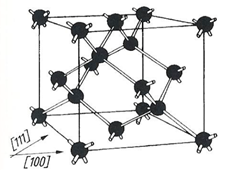
\includegraphics[width=0.5\textwidth]{Bilder/kap1/Diamant-GitterstrukturVonSilizium.png}
        \caption{\textbf{Diamantgitterstruktur von Silizium}}  
        %\label{fig:Diamant-GitterstrukturVonSilizium}
    \end{figure}
    }

    %Gesprochener Text:
    %%
\end{frame}

%Zinkblende-Gitterstruktur von GaAs
\begin{frame}
    \b{
    \frametitle{Halbleitermaterialien}
    \begin{figure}[H]
        \centering
        %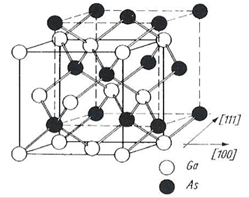
\includegraphics[width=0.5\textwidth]{Bilder/kap1/Zinkblende-GitterstrukturVonGaAs.png}
        \begin{minipage}[c]{0.48\textwidth}
            \centering
            \includesvg[width=0.7\textwidth]{Bilder/kap1/Gitterstrukturen/GitterGaAs_1}
        \end{minipage}
        \begin{minipage}[c]{0.48\textwidth}
            \centering
            \includesvg[width=0.7\textwidth]{Bilder/kap1/Gitterstrukturen/GitterGaAs_2}
        \end{minipage}
        \caption{\textbf{Zinkblende-Gitterstruktur von GaAs}}  
        %\label{fig:Zinkblende-GitterstrukturVonGaAs}
    \end{figure}
    }

    %Gesprochener Text:
    %%
\end{frame}

%Merke
\begin{frame}
    \b{
    \frametitle{Halbleitermaterialien}
    \textbf{Merke:}
    \begin{itemize}
        \onslide<1->{
        \item Silizium ist das am weitesten verbreitete Halbleitermaterial.
        }
        \onslide<2->{
        \item Verbindungshalbleiter bestehen aus zwei Materialen die in bestimmter Kombination Halbleiterverhalten aufweisen.
        }
        \onslide<3->{
        \item Silizium ist aus der IV. Hauptguppe des Periodensystem, Verbindungshalbleiter typischerweise aus der III. und V. Hauptguppe.
        }
    \end{itemize}}
% %Gesprochener Text:
% %speech{Einführung Halbleiterbauelemente}{1}{Halbleiterbauelemente sind das Rückgrat der modernen Elektronik und entscheidend für die Funktion vieler elektronischer Geräte, von Computern und Mobiltelefonen bis hin zu Solarzellen. Diese Bauelemente nutzen die besonderen Eigenschaften von Materialien, die weder gute Leiter noch gute Isolatoren sind, sondern dazwischen liegen, die sogenannten Halbleiter. Der Text beschreibt zunächst ihre Funktionsweise mit dem Bändermodell, das die elektronischen Zustände in Festkörpern erklärt, und untersucht dann verschiedene Halbleitermaterialien, ihre Eigenschaften und Anwendungen. Ein Schlüsselkonzept ist der pn-Übergang, der die Basis für viele Bauelemente bildet. Im zweiten Teil werden verschiedene Halbleiterbauelemente wie Dioden und Transistoren und deren Funktionen erläutert.}}
\end{frame}

%Tabelle Halbleiter Folie 1
\begin{frame}
    \b{
        \frametitle{Halbleitermaterialien}
        \begin{table}[H]
            \centering 
            \begin{tabular}{|p{1.7cm}|p{1.2cm}|p{2cm}|p{2.2cm}|p{2.2cm}|p{2.3cm}|}
                \hline
                \textbf{Material} & \textbf{Band- \newline lücke \newline (eV)} & \textbf{Ladungs- \newline trägerdichte \newline (cm$^{-3}$)} & \textbf{Elektronen- \newline beweglichkeit \newline (cm$^2$/Vs)} & \textbf{Löcher- \newline beweglichkeit \newline (cm$^2$/Vs)} & \textbf{Anwendungen}\\
                \hline
                Si  & 1,1 & $10^{10} - 10^{15}$ & 1500 & 450 & Mikrochips, \newline Solarzellen, Sensoren \\
                \hline
                Ge & 0,7 & $10^{13} - 20^{19}$ & 3900 & 1900 & Transistoren, \newline Infarot-Detektoren \\
                \hline
                GaAs & 1,43 & $10^6 - 10^8$ & 8500 & 400 & Hochfrequenz- schaltungen, LEDs, Laserdioden \\
                \hline
                \end{tabular}
                \caption{Eigenschaften verschiedener Halbleitermaterialien}
                %\label{tab:EigenschaftenVerschiedenerHalbleitermaterialien}
        \end{table}
    }

    %Gesprochener Text:
    %%
\end{frame}

%Tabelle Halbleiter Folie 1
\begin{frame}
    \b{
        \frametitle{Halbleitermaterialien}
        \begin{table}[H]
            \centering 
            \begin{tabular}{|p{1.7cm}|p{1.2cm}|p{2cm}|p{2.2cm}|p{2.2cm}|p{2.3cm}|}
                \hline
                \textbf{Material} & \textbf{Band- \newline lücke \newline (eV)} & \textbf{Ladungs- \newline trägerdichte \newline (cm$^{-3}$)} & \textbf{Elektronen- \newline beweglichkeit \newline (cm$^2$/Vs)} & \textbf{Löcher- \newline beweglichkeit \newline (cm$^2$/Vs)} & \textbf{Anwendungen}\\
                \hline
                InP & 1,35 & $10^{16} - 10^{17}$ & 5000 - 7000 & 200 - 400 & Optoelektronik, \newline Solarzellen \\
                \hline 
                GaN & 3,4 & $10^{13} - 10^{17}$ & 1000 - 2000 & 50- 200 & Leistungs- \newline elektronik, LED-Beleuchtung, Displays \\
                \hline
                SiC & 3,0 & $10^{12} - 10^{16}$ & 800 - 1200 & 200 - 400 & Leistungs- \newline eletronik, \newline Hochtemperatur- \newline anwendung \\ 
                \hline
                \end{tabular}
                \caption{Eigenschaften verschiedener Halbleitermaterialien}
                %\label{tab:EigenschaftenVerschiedenerHalbleitermaterialien}
        \end{table}
    }

    %Gesprochener Text:
    %%
\end{frame}

%Gitterstruktur und Bändermodell von Si - Abbildung 8
\begin{frame}
    \b{
    \frametitle{Ladungsträgertransport}
    \onslide<1->{
    \begin{minipage}[t]{0.48\textwidth}
        \begin{figure}[H]
            \centering
            \includesvg[width=\textwidth]{Bilder/kap1/GitterstrukturUndBaendermodellVonSi/GitterstrukturUndBaendermodellVonSi_1}
            \caption{\textbf{Gitterstruktur und Bändermodell von Si} reines Silizium bei T $=$ 0 K}  
            \label{fig:GitterstrukturUndBaendermodellVonSi-1}
        \end{figure}
    \end{minipage}
    }
    \onslide<2->{
    \begin{minipage}[t]{0.48\textwidth}
        \begin{figure}[H]
            \centering
            \includesvg[width=\textwidth]{Bilder/kap1/GitterstrukturUndBaendermodellVonSi/GitterstrukturUndBaendermodellVonSi_2}
            \caption{\textbf{Gitterstruktur und Bändermodell von Si} reines Silizium bei T $>$ 0 K}  
            \label{fig:GitterstrukturUndBaendermodellVonSi-2}
        \end{figure}
    \end{minipage}
    }
    }

    %Gesprochener Text:
    %%
\end{frame}

%Gitterstruktur und Bändermodell von n-dotiertem Si - Abbildung 9
\begin{frame}
    \b{\frametitle{Ladungsträgertransport}
    \onslide<1->{
        \begin{minipage}[t]{0.48\textwidth}
            \begin{figure}[H]
                \centering
                \includesvg[width=\textwidth]{Bilder/kap1/GitterstrukturUndBaendermodellVonN-dotiertesSi/GitterstrukturUndBaendermodellVonN-dotiertesSi_1}
                \caption{\textbf{Gitterstruktur und Bändermodell von n-dotiertem Si} n-dotierts Silizium bei T $=$ 0 K.}  
                \label{fig:GitterstrukturUndBaendermodellVonN-DotiertesSi-1}
            \end{figure}
        \end{minipage}
    }
    \onslide<2->{
        \begin{minipage}[t]{0.48\textwidth}
            \begin{figure}[H]
                \centering
                \includesvg[width=\textwidth]{Bilder/kap1/GitterstrukturUndBaendermodellVonN-dotiertesSi/GitterstrukturUndBaendermodellVonN-dotiertesSi_2}
                \caption{\textbf{Gitterstruktur und Bändermodell von n-dotiertem Si} n-dotierts Silizium bei T $>$ 0 K.}  
                \label{fig:GitterstrukturUndBaendermodellVonN-DotiertesSi-2}
            \end{figure}
        \end{minipage}
    }
    }

    %Gesprochener Text:
    %%
\end{frame}

%Gitterstruktur und Bändermodell von p-dotiertem Si
\begin{frame}
    \b{\frametitle{Ladungsträgertransport}
    \onslide<1->{
    \begin{minipage}[t]{0.48\textwidth}
        \begin{figure}[H]
            \centering
            \includesvg[width=\textwidth]{Bilder/kap1/GitterstrukturUndBaendermodellVonP-dotiertesSi/GitterstrukturUndBaendermodellVonP-dotiertesSi_1}
            \caption{\textbf{Gitterstruktur und Bändermodell von p-dotiertem Si} p-dotierts Silizium bei T $=$ 0 K.}  
            \label{fig:GitterstrukturUndBaendermodellVonP-DotiertesSi-1}
        \end{figure}
    \end{minipage}
    }
    \onslide<2->{
    \begin{minipage}[t]{0.48\textwidth}
        \begin{figure}[H]
            \centering
            \includesvg[width=\textwidth]{Bilder/kap1/GitterstrukturUndBaendermodellVonP-dotiertesSi/GitterstrukturUndBaendermodellVonP-dotiertesSi_2}
            \caption{\textbf{Gitterstruktur und Bändermodell von p-dotiertem Si} p-dotierts Silizium bei T $>$ 0 K.}  
            \label{fig:GitterstrukturUndBaendermodellVonP-DotiertesSi-2}
        \end{figure}
    \end{minipage}
    }
    }

    %Gesprochener Text:
    %%
\end{frame}

%Merke
\begin{frame}
    \b{
    \frametitle{Ladungsträgertransport}
    \textbf{Merke:}
    \begin{itemize}
        \onslide<1->{
        \item Durch thermische Anregung können freie Elektronen entstehen, die zum Ladungsträgertransport beitragen. 
        } \onslide<2->{
        \item Dotierung ist das gezielte Einbringen von Fremdatomen mit oder weniger Valenzelektronen als das Ausgangsmaterial.
        } \onslide<3->{
        \item Für n-Dotierung kann Phosphor und für p-Dotierung Bor genutzt werden.
        }
    \end{itemize}}
% %Gesprochener Text:
% %speech{Einführung Halbleiterbauelemente}{1}{Halbleiterbauelemente sind das Rückgrat der modernen Elektronik und entscheidend für die Funktion vieler elektronischer Geräte, von Computern und Mobiltelefonen bis hin zu Solarzellen. Diese Bauelemente nutzen die besonderen Eigenschaften von Materialien, die weder gute Leiter noch gute Isolatoren sind, sondern dazwischen liegen, die sogenannten Halbleiter. Der Text beschreibt zunächst ihre Funktionsweise mit dem Bändermodell, das die elektronischen Zustände in Festkörpern erklärt, und untersucht dann verschiedene Halbleitermaterialien, ihre Eigenschaften und Anwendungen. Ein Schlüsselkonzept ist der pn-Übergang, der die Basis für viele Bauelemente bildet. Im zweiten Teil werden verschiedene Halbleiterbauelemente wie Dioden und Transistoren und deren Funktionen erläutert.}}
\end{frame}

%Driftstrom Innerhalb Eines Halbleiters
\begin{frame}
    \b{
    \frametitle{Ladungsträgertransport}
    \begin{figure}[H]
        \centering
        \includesvg[width=0.5\textwidth]{Bilder/kap1/DriftstromInnerhalbEinesHalbleiters}
        \caption{\textbf{Driftstrom innerhalb eines Halbleiters}}  
        %\label{fig:DriftstromInnerhalbEinesHalbleiters}
    \end{figure}
    }

    %Gesprochener Text:
    %%
\end{frame}

%Diffusions Innerhalb Eines Halbleiters
\begin{frame}
    \b{
    \frametitle{Ladungsträgertransport}
    \begin{figure}[H]
        \centering
        \includesvg[width=0.8\textwidth]{Bilder/kap1/DiffusionsstromInnerhalbEinesHalbleiters}
        \caption{\textbf{Diffusionsstrom innerhalb eines Halbleiters}}  
        %\label{fig:DiffusionsstromInnerhalbEinesHalbleiters}
    \end{figure}
    }

    %Gesprochener Text:
    %%
\end{frame}

%Einfluss von Spannungen auf Halbleiter
\begin{frame}
    \b{
    \frametitle{Ladungsträgertransport}
    \begin{figure}[H]
        \centering
        \includesvg[width=0.8\textwidth]{Bilder/kap1/EinflussvonSpannungenaufHalbleiter}
        \caption{\textbf{Einfluss von Spannungen auf Halbleiter}}  
        %\label{fig:EinflussVonSpannungenAufHalbleiter}
    \end{figure}
    }

    %Gesprochener Text:
    %%
\end{frame}

%Merke
\begin{frame}
    \b{
    \frametitle{Ladungsträgertransport}
    \textbf{Merke:}
    \begin{itemize}
        \onslide<1->{
        \item Driftstrom ist der Ladungsträgertransport auf Grund eines elektrischen Feldes.
        } \onslide<2->{
        \item Diffusionsstrom ist die Bewegung von Ladungsträgern auf Grund eines Konzentrationsunterschiedes.
        } \onslide<3->{
        \item Drift- und Diffusionsstrom ergeben zusammen den Gesamtstrom.
        } \onslide<4->{
        \item Eine externe Spannung führt zu einer Verschiebung des Bändermodells. 
        }
    \end{itemize}}
% %Gesprochener Text:
% %speech{Einführung Halbleiterbauelemente}{1}{Halbleiterbauelemente sind das Rückgrat der modernen Elektronik und entscheidend für die Funktion vieler elektronischer Geräte, von Computern und Mobiltelefonen bis hin zu Solarzellen. Diese Bauelemente nutzen die besonderen Eigenschaften von Materialien, die weder gute Leiter noch gute Isolatoren sind, sondern dazwischen liegen, die sogenannten Halbleiter. Der Text beschreibt zunächst ihre Funktionsweise mit dem Bändermodell, das die elektronischen Zustände in Festkörpern erklärt, und untersucht dann verschiedene Halbleitermaterialien, ihre Eigenschaften und Anwendungen. Ein Schlüsselkonzept ist der pn-Übergang, der die Basis für viele Bauelemente bildet. Im zweiten Teil werden verschiedene Halbleiterbauelemente wie Dioden und Transistoren und deren Funktionen erläutert.}}
\end{frame}

\begin{frame}
    \b{
    \frametitle{pn-Übergang}
    \begin{figure}[H]
        \centering
        \includesvg[width=\textwidth]{Bilder/kap1/FolienVorgaengeInnerhalbeinesPNUebergangs1}
        \caption{\textbf{Vorgänge innerhalb eines pn-Übergangs.}}  
        %\label{fig:VorgaengeInnerhalbEinesPn-Uebergangs1}  
    \end{figure}
    }

\end{frame}

\begin{frame}
    \b{
    \frametitle{pn-Übergang}
    \begin{figure}[H]
        \centering
        \includesvg[width=0.6\textwidth]{Bilder/kap1/FolienVorgaengeInnerhalbeinesPNUebergangs2}
        \caption{\textbf{Vorgänge innerhalb eines pn-Übergangs.} }  
    \end{figure}
          \begin{itemize}
            \onslide<1->{
        \item Durch die Bindung der Löcher und Elektronen an deren Atome begrenzt den Diffusionsstrom.
            } \onslide<2->{
        \item Der Bereich in der Mitte nennt sich Raumladungszone (RLZ). Dort sind keine freien Ladungsträger, da die Elektronen und Löcher sich gegenseitig neutralisieren.
            } \onslide<3->{
        \item Es entsteht ein elektrisches Feld zwischen den p- und n-dotierten Bereichen.
            }
    \end{itemize}
    }

\end{frame}

%Vorgänge innerhalb des pn-Übergangs.
\begin{frame}
    \b{
    \frametitle{pn-Übergang}
    \begin{figure}[H]
        \centering
        \includesvg[width=\textwidth]{Bilder/kap1/VorgaengeInnerhalbDesPN-Uebergangs}
        \caption{\textbf{Vorgänge innerhalb des pn-Übergangs.}}  
        %\label{fig:VorgaengeInnerhalbDesPn-Uebergangs}
    \end{figure}
    }

    %Gesprochener Text:
    %%
\end{frame}

%Einfluss von Spannungen auf pn-Übergang.
\begin{frame}
    \b{
    \frametitle{pn-Übergang}
    \begin{figure}[H]
        \centering
        \includesvg[width=0.7\textwidth]{Bilder/kap1/EinflussvonSpannungenaufpn-Uebergang}
        \caption{\textbf{Einfluss von Spannungen auf pn-Übergang.} Raumladungszone bei verschiedenen angelegten Spannungen. Links: Spannung in Durchlassrichtung. Rechts: Spannung entgegen der Durchlassrichtung, Sperrrichtung}  
        %\label{fig:EinflussVonSpannungenAufPn-Uebergang}
    \end{figure}
    }

    %Gesprochener Text:
    %%
\end{frame}

%Merke
\begin{frame}
    \b{
    \frametitle{pn-Übergang}
    \textbf{Merke:}
    \begin{itemize}
        \onslide<1->{
        \item Der pn-Übergang kombiniert eine p- und n-dotierte Halbleiterschicht.
        } \onslide<2->{
        \item Im Übergangsbereich sind keine freien Ladungsträger, der Bereich wird Raumladungszone genannt.
        } \onslide<3->{
        \item In Durchlassrichtung wird die RLZ verkleinert, in Sperrrichtung wird diese vergrößert.  
        }
    \end{itemize}}
% %Gesprochener Text:
% %speech{Einführung Halbleiterbauelemente}{1}{Halbleiterbauelemente sind das Rückgrat der modernen Elektronik und entscheidend für die Funktion vieler elektronischer Geräte, von Computern und Mobiltelefonen bis hin zu Solarzellen. Diese Bauelemente nutzen die besonderen Eigenschaften von Materialien, die weder gute Leiter noch gute Isolatoren sind, sondern dazwischen liegen, die sogenannten Halbleiter. Der Text beschreibt zunächst ihre Funktionsweise mit dem Bändermodell, das die elektronischen Zustände in Festkörpern erklärt, und untersucht dann verschiedene Halbleitermaterialien, ihre Eigenschaften und Anwendungen. Ein Schlüsselkonzept ist der pn-Übergang, der die Basis für viele Bauelemente bildet. Im zweiten Teil werden verschiedene Halbleiterbauelemente wie Dioden und Transistoren und deren Funktionen erläutert.}}
\end{frame}
